\chapter[Computational Model]{Computational Model}
\label{chap:computational_model}

\lettrine{F}{or} a computer to express accommodative speech, a machine-understandable description of the process is required.
This chapter introduces a model of the accommodation process in humans, based on the finding in the human-human and human-computer studies presented in previous chapters.
It's motivated by empirical data observed in these studies and aims to resemble the process that occurs in humans.
The human-centric insiprations and the parameters representing them are discussed and demonstrated.

\pagebreak

\acresetall

\section{From \acs{hhi} to \acs{hci}}
\label{sec:from_hhi_to_hci}

The experiments presented in \cref{part:experiments} show humans' accommodation behaviors in different \acf{hhi} and \acf{hci} settings.
Complementary to those, \cref{subsec:accommodation_levels} discusses ways to represent the various levels of accommodative behaviors in computers.
Since behavioral changes, as explained by \ac{cat} (see \cref{sec:communication_accommodation_theory}), happen naturally and often unconsciously in \ac{hhi}, it is not trivial to transfer them to computers, as they need defined rules and numeric representation to process.
Numeric values can be achieved by applying some measuring technique appropriate for each feature, like formant values for vowel quality or frequency for \ac{f0}.
Rules for different behaviors, however, cannot be directly constructed, due to the intuitive nature of this inherent phenomenon, but can instead be inferred from observed \ac{hhi} data.
For example, the results of the study described in \cref{chap:shadowing_in_sung_music_and_human_computer_interaction} reveal a high degree of variation across participants (\cref{subsec:results_hci}).
While this is expected, further examination of these variations uncovers some general properties that can be taken as a basis for characterizing the different changes.
The link between the measured raw values and systematic rules should be a machine-applicable equivalence of the accommodation process in humans.
Such parallelisms would need to model, for instance, the way humans percept accommodation-prone sounds, how they interact with previous instances and the current internal state of the sound in question, and the cognitive process of the phonetic changes.
Therefore, such a model should include the perception of the phonetic features, representation of the state change of each feature in memory, and the realization of the changes during a conversation.
Since these steps are dependent on each other, the computational model presented here is depicted as a pipeline, in which each of its steps stands for one of the sub-processes mentioned above.

\section{Pipeline representation}
\label{sec:pipeline_representation}

As accommodation happens automatically and seamlessly in human interlocutors' cognition, it is hard to say what are the exact steps this process comprises.
Some key properties stand out when examining many occurrences in different interactions.
The pipeline presented here aims to capture these properties and offer a defined process of describing the changes.
The advantages of representing this process as a pipeline (as opposed to, e.g., a one-step, end-to-end conversion) is that each facet of the process can be interpreted and controlled separately (as demonstrated in \cref{subsec:computational_model,fig:adaptation_module_pipeline}).
This enables combining and experimenting with different methods and implementations for each step while maintaining their independence of each other.
The ability to substitute a single step's logic without influencing ther others grants the freedom to experiment with different methods without losing the core principles of the accommodation process.
For example, the calculation method in the \textit{update} step can be changed or even replaced by a statistical model (like the one introduced in \cref{chap:statistical_model}).
Note that although only speech-related features are discussed here, this pipeline could be used for describing changes in other types of features and modalities, such as lexical choices, linguistic complexity, eye gaze, emotional state, etc.

The proposed pipeline representation consists of the following five main steps, which are explained in detail in \crefrange{subsec:detect}{subsec:assign}:
%
\begin{itemize}[topsep=0cm, itemsep=-.1cm, wide=0cm, leftmargin=!, labelwidth=\widthof{\textbf{update}}]
	\item[\textbf{detect}] hear and identify a feature that can be changed, corresponding to a human ear's ability to notice such variations;
	
	\item[\textbf{filter}] decide whether the encountered feature's instance appears in a way that can trigger change, capturing the inherent detection of phonological context and rules in the language;
	
	\item[\textbf{store}] add the instance to the exemplar pool of this feature, representing the inventory that builds the internal representation of the feature;
	
	\item[\textbf{update}] update the feature's state, standing for the \enquote{recalculation} of the way this feature is perceived by the speaker; and
	
	\item[\textbf{assign}] apply and potentially limit the updated state, expressing the change in a speaker's production of this feature with the individual preference as to how far to go with a change.
\end{itemize}
%
The output of each step is the direct input for the next, except for cases where the execution is discontinued due to an unmet condition (see \cref{fig:adaptation_module_pipeline}).
%
\begin{figure}[t]
	\centering
	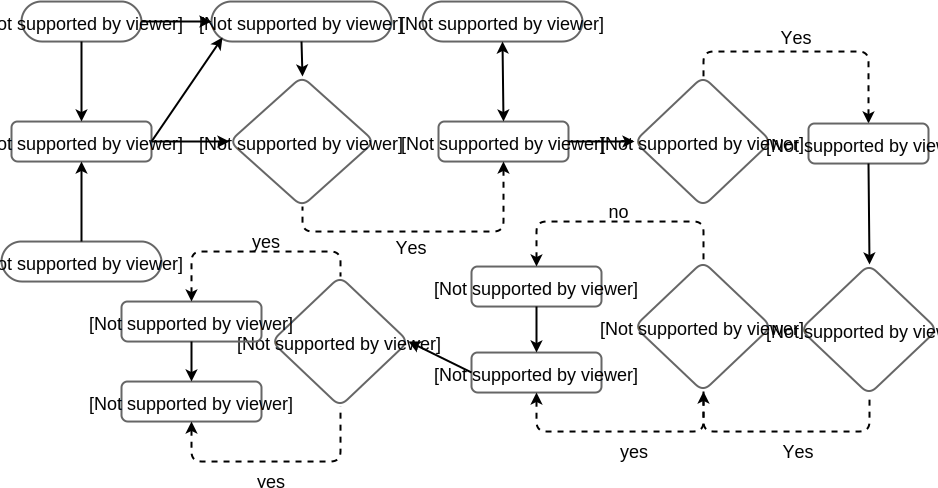
\includegraphics[width=\linewidth]{pipeline}
	\caption[Phonetic convergence algorithm pipeline]
		{Overview of the vocal accommodation pipeline.
		Rectangle nodes represent steps where an action is performed, round rectangles are inputs (either external or from the system), and diamond-shaped nodes stand for decision points.
		Nodes without a \enquote{no} edge indicate termination of the process at that point if their condition is not met (and therefore no accommodation takes place).
		The pipeline is successfully completed only once the \enquote{Set feature's new value} node is reached.}
		% However, if the \enquote{Add exemplar} action was performed prior to termination, the exemplar is not removed and will be taken into consideration the next time the pipeline is triggered for the feature with which it is associated.
		% The \enquote{feature definitions} come from the configuration file and can be changed by the user.}
	\label{fig:adaptation_module_pipeline}
\end{figure}

\subsection{Detect}
\label{subsec:detect}

This step stands for the human ability to identify phonemes in speech and analyze the way they are realized.
The input to this first step in the pipeline is the raw speech signal of the speaker and its output is a sequence of realizations that may contain phonetic changes.
The \ac{asr} component of the system is responsible for detecting these realizations and their timestamps in the signal.
With this information, various methods can be used to define and measure target features to take into consideration and pass forward.
\Cref{subsubsec:detecting_segment_exemplars} shows an example of such a definition and how it is used in a \ac{sds}.

An interlocutor cannot accommodate to features that are not present in a speaker's speech.
For changes on any level to happen, some pre-defined feature that is prone to change needs to be present and detected in the input speech stream.
Moreover, for the changes to register as a variation of a feature, the realization produced by the speaker must be prominent and distinctive enough to be perceived by the listener.
In the case of computers, that means a way to measure the difference between realizations and classify their distance from one another.
This difference can be categorical or continual, depending on the feature.
In addition, not only the features which introduce meaningful difference are language- and culture-dependent, but they might also differ based on the specific situation in which the interaction takes place.
For example, a segmental feature of a language where a phoneme can be realized in two alternative ways (as the allophonic alteration explained in \cref{subsubsec:target_features_HCIConv}) will probably be ignored by a speaker of a language where only one of these vowels exist in its repository.
In this case, the two vowels will simply be mentally merged into one, without causing any difficulties with comprehension.
Suprasegmental features, like \ac{f0} contour and \ac{ar}, occur globally across the speech signal and are more often cross-lingual.
Still, for a computer to be able to detect and track changes in those features, a way to measure and compare them is required.

\subsection{Filter}
\label{subsec:filter}

This step corresponds the human internal, often unconscious, linguistic knowledge, and how it is used to decide which detected realizations are valid new instances that will be stored in memory.
Its input is instances of a defined target feature detected in the previous step and it outputs those instances that should be stored as exemplars of their respective features.
\Cref{subsubsec:filtering_exemplars} demonstrates how a filter is applied based on a phonological rule and a feature definition with a target phoneme.

A target phoneme serves as an anchor for a rule that aims to capture a phonetic feature or a more evolved phonological rule.
For example, the German phonological rule of \textipa{[@]} elision at word-final \emph{-en} (as described by \cref{eq:schwa_elision_rule}) can be captured by the phoneme sequence /C\textipa{@n}/, where C represents a consonant (although in practice only a subset of the German consonants inventory can be placed at this position).
The anchor phoneme is \textipa{[@]}, since this is the segment that is subject to the change, namely the length -- or complete absence -- of it.
therefore, for this phenomenon, the target phoneme would be \textipa{[@]} and the measured feature would be segment length.
Another target feature described in \cref{subsubsec:target_features_HCIConv} is \textipa{[e:]} vs.\ \textipa{[E:]} realization of the mid-word grapheme \emph{ä}, which is captured by the target anchor phoneme \textipa{[E]} in a non-final position of a word.
Any defined feature goes through two filters.
First, the phonological context of the detected sequence is matched against the one defined for the target feature; and secondly, the defined accepted value range that would make it an acceptable instance of that phenomenon, like \textipa{[@]} length between \SI{0}{\milli\second} and \SI{60}{\milli\second} or appropriate F$_1$ and F$_2$ values for the \textipa{[e:]} and \textipa{[E:]} vowels in the aforementioned features.
After applying these two filters, only those instances that truthfully capture the desired phonetic phenomenon are kept.
Another purpose of this step is to provide a way to integrate phonetic expertise to be used in the process.
This helps not only to be more accurate regarding language-specific knowledge, but also to prevent \ac{asr} errors to propagate further in the pipeline.

\subsection{Store}
\label{subsec:store}

\begin{figure}[t]
	\centering
	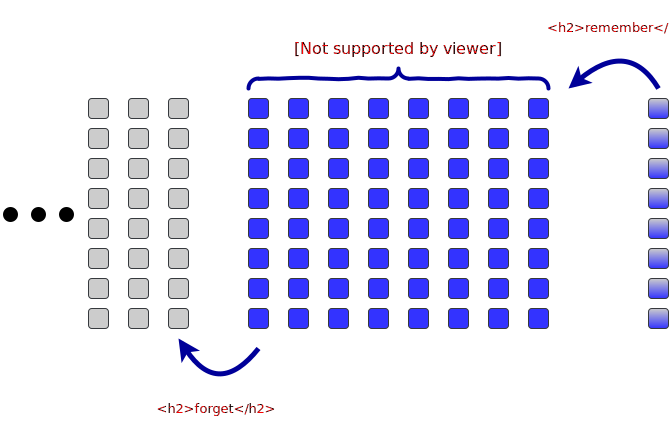
\includegraphics[width=0.7\textwidth]{pool}
	\caption[The exemplar pool]
		{Illustration of an exemplar pool.
		Each exemplar is represented by a column of squares (each representing a numeric value).
		A new exemplar is added to the feature's pool when encountered.
		Old exemplars are removed when the pool is full.
		Exemplars currently in the pool are taken into account when the realization of the feature is determined.}
	\label{fig:exemplar_pool}
\end{figure}
%
This step represents the mental phonetic memory of a speaker, here referred to as a \emph{pool} for a computer-based interlocutor.
The input to it is a feature's exemplars that passed the filtering step and its output is used for updating the feature's representation.
An illustration of an exemplar pool is shown in \cref{fig:exemplar_pool} and an implementation of it is described in \cref{subsubsec:collecting_exemplars}.

After an instance of a feature is detected and validated, it needs to be registered as an exemplar of the feature it is associated with.
This stands in parallel to the way such exemplars (and in other contexts also words, meanings, etc.) are mentally stored in the human's short- and long-term memories.
These accumulated exemplars of a feature determine how a speaker perceives it and shape its production when used in speech.
One of the complexities of modeling such internal representation is the interleaving influences of both long-term and short-term memory.
In spoken interaction, the long-term memory may define the typical productions of a user, while the short-term memory is used and changed within a single conversation.
Since this model aims to describe accommodation occurring within the scope of a single, isolated interaction (even if a long one), only the storage of exemplars encountered in this interaction is explicitly addressed in it.
However, long-term effects may be implicitly achieved by retaining values between interactions.
This step also defines how new exemplars are added, stored, and removed (cf.\ \cref{fig:exemplar_pool}).
Each feature has its own exemplar pool to which newly encountered exemplars are \enquote{memorized}, and each exemplar is a vector of the values measured for the target feature, e.g., formant values).
The pool functions in a first-in-first-out fashion, fitting the temporally linear progression of spoken interaction.
An exemplar is represented by a vector with cardinality $n$, where $n$ is the number of dimensions required for describing this feature.
Whenever an exemplar of the feature is encountered, a new exemplar is added to the pool.
The size of the pool determines the memory capacity, i.e., for how long exemplars are remembered during the interaction.
If the pool is already at full capacity, the oldest exemplar is \enquote{forgotten} when a new exemplar is added.
Ultimately, a pool of a feature can be used to determine which exemplars are still affecting the speaker's mental state of a feature.
As the order of the added exemplars is kept, it can be taken into account as well when determining each exemplar's weight, just like recent turns are more likely to influence the current utterance than turns from the beginning of the conversation.

\subsection{Update}
\label{subsec:update}

This step incorporates the process of changing the mental state of a feature based on its accumulated exemplars.
The input to it is the current state of a feature and it outputs a new value for it.

The core of the accommodation process is the change in a feature's state.
Many factors may influence this change, both internal and external.
The two main considerations in this step are one of each, namely the desired accommodation behavior and the exemplars collected from the user's speech input.
The latter is covered by the \enquote{store} step, and the former is defined using adjustable parameters that correspond to accommodation properties in humans (see \cref{tab:comp_model_parameters}).
For example, how prone is the speaker to be influenced by others' speech and how easily should the change be triggered.
The sensitivity can be constant or vary based, e.g., on how close are the speakers' productions to begin with.
A trigger might be exemplar-based, i.e., after a certain number of new exemplars were added, or time-based, i.e., every time a certain amount of turns had passed.
Another means to shape the behavior is the way the new state is computed based on the exemplars.
For example, newer exemplars or exemplars with greater distance from the current state may influence the change more.
Moreover, the general tendency to accommodate is defined in this step, e.g., converging or diverging from the user's speech, which is determined, among others, by the application and desired behavior.
A \ac{capt} system would probably not aim to align its speech to the user's, but rather diverge from it as a way to provide auditory feedback.
This computation can use simple mathematical operations (as demonstrated in \cref{subsubsec:calculating_changed_value}) or more involved data-driven statistical methods (as the one in \cref{chap:statistical_model}).

\subsection{Assign}
\label{subsec:assign}

This step mediates between the new state of a feature and its use in the system's speech output.
The input to it is the newly calculated state of a feature and it outputs a potentially altered version of this state to be used by the \ac{tts} component.

This final step of the pipeline is responsible for assigning the features' representations to the speech production of the system as an additional input to the system's \ac{tts} component.
For a \ac{tts} module that can directly control the speech output (as part of the model itself or on the outputted waveform, as discussed in \cref{subsec:speech_manipulation}),
this additional information can be used to manipulate the target features in a way that expresses the accommodative behavior of the system.
This closes the circle from a target feature produced by the user and up to the change it triggered in the system when it speaks back.
Since that means the user will now hear certain vocal characteristics that are based on their own speech, it is important to avoid a situation where the user feels imitated -- or even mocked -- by the systems.
This is an important issue that has not been considered in previous work.
To that end, this step introduces a limitation mechanism that limits the values given to the \ac{tts} component.
The values are re-evaluated if some threshold is bypassed (see \cref{eq:new_value}), to avoid such imitation from the system's side.
This mechanism also helps to prevent the system from diverging too sharply from the user.
For example, a \ac{capt} system might demotivate or frustrate the user if its speech is consistently considerably different from the user's.
From a human's perspective, this step corresponds to the natural degree to which a speakers would change their speech while talking to others.
As shown in \cref{chap:shadowing_in_sung_music_and_human_computer_interaction,chap:speech_variations_in_hhci}, this varies from feature to feature, and hence this parameter is set for each feature individually (see \cref{tab:comp_model_parameters}).
For this to work, it is important that the features are sufficiently distinguishable and clearly defined by the pipeline, so that the specified modification in the system's speech output can be properly applied in -- and only in -- the correct places, as illustrated in \cref{fig:adapted_synthesis_output}.
%
\begin{figure}[t]
	\centering
	\includegraphics[width=0.75\textwidth]{synthesis}
	\caption[Manipulated features on a synthesized waveform (illustration)]
		{Illustration of a manipulated output audio waveform.
		Each colored pin marks a phonetic features captured and processed by the pipeline.}
	\label{fig:adapted_synthesis_output}
\end{figure}

\section{Parameters}
\label{sec:parameters}

Several parameters are introduced into the pipeline described in \cref{sec:pipeline_representation} to grant degrees of freedom in shaping the accommodation behavior.
These parameters link between the theoretical, schematic model and its integration into a \ac{sds}, as demonstrated in \cref{chap:convergence_module_for_sdss}.
They are also the key to experimentation with different settings and scenarios for different applications.
The model's parameters are summarized in \cref{tab:comp_model_parameters} \citep[and cf.][]{Raveh2017Interspeech}.

\afterpage{%
	\begin{landscape}
		\begin{table}[t]
			\centering
			\vspace{1.5cm}
			\caption[Summary of computational model's parameters]
				{Computational model's parameters in their order of use.
				The colors mark parameters associates with the
				{\color{Violet}\textbf{detect}},
				{\color{BurntOrange}\textbf{filter}},
				{\color{ForestGreen}\textbf{store}},
				{\color{RoyalBlue}\textbf{update}}, and
				{\color{red}\textbf{assign}} steps.}
			\label{tab:comp_model_parameters}
			\begin{tabulary}{\linewidth}{lLL}
				\toprule
				\multicolumn{1}{c}{\textbf{Parameter}} & \multicolumn{1}{c}{\textbf{Description}} & \multicolumn{1}{c}{\textbf{Value}} \\
				
				{\color{Violet}\textbf{target phoneme}}*
				& the phoneme that triggers the feature's pipeline
				& a phoneme symbol\\\addlinespace[0.2cm]
				
				{\color{BurntOrange}\textbf{phonetic context}}*
				& the environment in which the feature instance is accepted
				& regex containing the of phoneme symbols containing target phoneme\\\addlinespace[0.2cm]
				
				{\color{BurntOrange}\textbf{allowed range}}*
				& the value range(s) in which new instances are accepted
				& two numeric values (min and max) per feature dimension\\\addlinespace[0.2cm]
				
				{\color{ForestGreen}\textbf{exemplar pool size}}
				& maximum number of exemplars in memory at a time, oldest exemplar removed when full
				& positive integer\\\addlinespace[0.2cm]
				
				{\color{RoyalBlue}\textbf{update frequency}}
				& how frequently a feature's value is recalculated, controlling the accommodation pace
				& non-negative integer; 0 for manual update\\\addlinespace[0.2cm]
				
				{\color{RoyalBlue}\textbf{calculation method}}*
				& the manner in which the pool value is calculated based on the values and order of the exemplars in pool
				& any $\mathbb{R}^{n \times m} \longrightarrow \mathbb{R}^{m}$ function; either implemented directly in code or sent to an external statistical model\\\addlinespace[0.2cm]
				
				{\color{RoyalBlue}\textbf{convergence rate}}
				& weight of the exemplar pool when updating the feature's state, controlling the impact of external input on the speaker's features states
				& real value; typically $n \in (0, 1) \subset \mathbb{R}$; 0 for ignoring the pool; $> 1$ for over-weighting the pool value\\\addlinespace[0.2cm]
				
				{\color{red}\textbf{convergence limit}}*
				& the maximum degree of convergence allowed for the feature with respect to the input instances
				& real value; $n \in (0, 1] \subset \mathbb{R}$; 1 (\SI{100}{\percent}) for no limitation \\
				\bottomrule
			\end{tabulary}
			\flushleft{\footnotesize \emph{* denotes parameters that are defined individually for each feature}}
		\end{table}
	\end{landscape}
}

As shown in \cref{sec:convergence_to_natural_and_synthetic_stimuli}, not all participants showed the same \emph{sensitivity} toward changes in the stimuli.
Here, sensitivity refers to the degree of overall change toward external speech input.
Additionally, when one does converge, the sensitivity to changes (i.e., the \enquote{amount of differentiation}) toward every single stimulus might differ as well.
These two aspects are jointly controlled by the \emph{convergence rate}, which represents the balance between the current and heard speech when calculating the accommodation outcome.
Generally, low convergence rate leads to a slow (and potentially unnoticeable) change, while a high rate would lead to sharper changes and that may overshoot the target, as demonstrated in \cref{tab:validation_baseline,fig:validation_sensitivity}.
To simulate the case where a speaker is not influenced by external speech input (the exemplars in the pool) at all, this rate can be set to zero.
In that case, the model will ignore the other interlocutor's speech and stick to the current speech style.
Another difference found among the participants was the total overall convergence degree toward the stimuli, i.e., where does the convergence process stop.
This is monitored by the \emph{convergence limit}, which defines the maximally allowed degree of similarity between the interlocutors.
When set to 1 (\SI{100}{\percent}), the model is allowed to change up to \SI{100}{\percent} toward the other interlocutor (complete convergence); when set to 0.8, up to \SI{80}{\percent}, and so on.
The parameter ensures that the model does not simply imitate the user's input, which is the approach often found in such system nowadays.
By limiting the change, the accommodation process is more gradual and restrained, avoiding peaks and abrupt changes.

Parameters defining the adaptation itself are not enough.
To properly model an accommodative behavior, some aspects that are not directly related to the speech output are required as well.
The accommodation process relies on the recent instances (\emph{exemplars}) of a speech sound.
How many exemplars are taken into account when the feature's state is updated depends on the interlocutor's mental memory of that sound.
This internal memory is a complex mechanism \citep{Baddeley2003working}, which is simplified here into a single parameter, namely the \emph{exemplar pool size}, which determines the number of exemplars the interlocutor currently remembers.
This exemplar history is managed on a first-in-first-out basis, so that the \emph{order} in which the exemplars were acquired is kept as well and can be used for weighting their influence.
This pool size can be tweaked to match the scenario and the expected interaction length.
The \emph{tendency to converge} toward other interlocutors also differs from speaker to speaker.
This likelihood is controlled by a parameter the parameter \emph{convergence rate}.
After an exemplar is added to a feature's pool, an update of the feature's value may be triggered.
Whether and how often this happens is determined by the \emph{update frequency}.
When set to 1, an update will occur every time an exemplar is added; if set to 2, every other exemplar, and so on.
When set to 0, however, updates will only take place when explicitly requested, e.g., after a pre-determined number of turns or a fixed amount of time.
This can be useful when all features are to be updated at the same time, regardless of how many exemplars have been accumulated for each of them.
Increasing the update interval means that each update will be affected by a higher number of new exemplars, which might result in a smoother converging process, depending on the calculation method used (see below).
Additionally, a longer update interval also means that accommodation will generally take longer, since the model's features are not being updated as frequently.
This is fitting for systems with which the user is expected to have long interactions.

Not only the frequency of updates plays a roll in the process, but also the manner in which the update is performed.
This manner is determined by the \emph{calculation method}.
Since the features in the model are represented by vectors, any function that takes a matrix as input and outputs a vector as output can be used, as demonstrated in \cref{subsubsec:calculating_changed_value}.
The method can be either statistical or deterministic, e.g., simply averaging the exemplars, but methods that can take order into account, like decaying average, might yield more realistic accommodative behaviors.
A different calculation method can be assigned to each feature, which can help to account for acoustic or psycholinguistic constraints.
This can also be influenced by the setting the system is purposed for, like experimental, exploratory, data collection, etc.

For each feature, a \emph{target phoneme} is defined, which serves two purposes:
First, it tells the \ac{asr} component which phoneme is associated with this feature, to later forward it for further analysis.
Secondly, it is used in the \emph{phonetic context} to filter instances of the phoneme that should not be associated with the feature.
The context is the environment in which the target phoneme should be found in the \ac{asr} output sequence for the instance to be considered\footnote{This requires an \ac{asr} engine that returns such a sequence in addition to textual output.
It is therefore crucial that the phoneme symbol set used in the model and by the \ac{asr} is the same and unambiguous, specifically when used in a regular expression.
This is the only part of the pipeline that is language-dependent (or rather symbol-dependent)
Using non-ASCII symbol sets, like IPA, may solve many of these issues, but is not recommended since \ac{asr} engines rarely use thoseת and also due to other technical reasons.}.
For suprasegmental features -- or any other feature that is not bound to a specific phoneme or context -- the target phoneme can remain empty, so that the phonetic context would match any sequence.
The second parameter used to put constrains on the detected phones is the \emph{allowed range}, which defines the minimum and maximum acceptable values for the feature.
This parameter is important to obtain clean and sensible exemplars, as it introduces restrictions based on phonetic knowledge (e.g., reasonable \ac{f0} values for a human speaker), which at the same time also help to prevent \ac{asr} errors from meddling with the exemplars sent to the pool.
Since these values are feature-dependent, this parameter is set for each feature individually.
%\Cref{subsubsec:detecting_segment_exemplars} shows an example of a feature definition.